\Subhead{3.2.1}{Теорема Винера--Хинчина. Белый шум и другие примеры спектров и корреляционных функций}

Для вещественного центрированного стационарного процесса используем двусторонний спектр по угловой частоте:
\begin{equation}\label{eq:wienerkhinchin}
 S_X(\omega)=\int_{-\infty}^{\infty}C_X(\tau)\e^{\ii\omega\tau}\dd\tau,
 \quad C_X(\tau)=\frac1{2\pi}\int_{-\infty}^{\infty}S_X(\omega)\e^{-\ii\omega\tau}\dd\omega.
\end{equation}
Это теорема Винера–Хинчина. Для конечной записи $X_T(\omega)=\int_{-T/2}^{T/2}X(t)\e^{\ii\omega t}\dd t$ раскрываем $\langle|X_T|^2\rangle$: стационарность заменяет двухвременное среднее на $C_X(t-s)$. Деление на $T$ даёт интеграл Фурье с треугольным весом $1-|\tau|/T$; при подходящей сходимости и $T\to\infty$ получаем $S_X$. Поэтому спектр неотрицателен, а
\begin{equation}
 \sigma_X^2=C_X(0)=\frac1{2\pi}\int S_X(\omega)\dd\omega.
\end{equation}
Реальный спектральный анализатор имеет конечное время и окно: оценка спектра сглаживается, её разброс требует усреднения, а узкие линии уширяются.

Белый шум: $C_X(\tau)=N\delta(\tau)$, $S_X=N$. Он является обобщённым процессом с бесконечной точечной дисперсией; физический шум белый лишь в ограниченной полосе. Экспоненциальная ковариация $C=\sigma^2\e^{-|\tau|/\tau_c}$ даёт лоренцев спектр $S=2\sigma^2\tau_c/[1+(\omega\tau_c)^2]$. Узкий спектр соответствует длинной корреляции. Для гармоники со случайной равномерной фазой $C=A^2\cos\omega_0\tau/2$, спектр состоит из двух дельта-линий. Шум $1/f$ нуждается в нижнем и верхнем срезах, иначе интегральная дисперсия расходится.

Односторонняя плотность по частоте в герцах $G_X(f)$, $f>0$, определяется равенством $\sigma^2=\int_0^\infty G_X(f)\dd f$. При наших соглашениях $G_X(f)=2S_X(2\pi f)$. Ошибка в этом переходе создаёт типичные множители $2$ и $2\pi$.
\begin{center}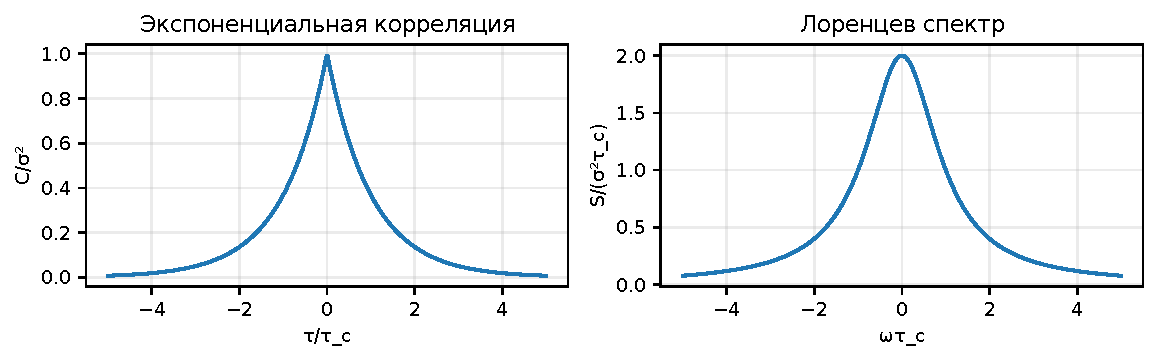
\includegraphics[width=0.8\linewidth]{figures/noise_spectrum.pdf}\end{center}

